\documentclass[11pt,letterpaper]{article}

\usepackage[NoDate]{currvita}
\usepackage{fullpage,mathpazo,hyperref,xcolor,graphicx}

\renewcommand{\cvheadingfont}{\bfseries\itshape\Huge}
\renewcommand{\cvlistheadingfont}{\bfseries\itshape\Large}
\hypersetup{colorlinks,breaklinks,urlcolor=cyan,linkcolor=cyan}

\begin{document}
\begin{cv}{Luis Alejandro Mart\'inez Faneyth}
\vspace{1em}

\begin{minipage}{.7\linewidth}
\begin{cvlist}{}
\item[\textit{\large{nacimiento}}]{Caracas, Venezuela --- 26 de Julio de 1986}
\item[\textit{\large{email}}]{\href{mailto:luis@huntingbears.com.ve}{luis@huntingbears.com.ve}}
\item[\textit{\large{blog}}]{\href{http://huntingbears.com.ve/}{huntingbears.com.ve}}
\item[\textit{\large{github}}]{\href{http://github.com/HuntingBears}{github.com/HuntingBears}}
\item[\textit{\large{gitorious}}]{\href{http://gitorious.org/~huntingbears}{gitorious.org/$\sim$huntingbears}}
\item[\textit{\large{deviantart}}]{\href{http://martinezfaneyth.deviantart.com/}{martinezfaneyth.deviantart.com}}
\end{cvlist}
\end{minipage}
\begin{minipage}{.3\linewidth}
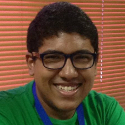
\includegraphics{curriculumvitae.jpg}
\end{minipage}
\vspace{1em}

\begin{cvlist}{Formaci\'on acad\'emica}
\item[{\parbox[t]{6em}{\textit{\large{2011}}}}]{
	\parbox[t]{\linewidth}{
		\textbf{Centro Nacional de Adistramiento} --- Caracas, Venezuela\\
		\textit{Administraci\'on del tiempo y productividad laboral} --- 16 Horas\\
		\footnotesize{T\'ecnicas organizativas, trabajo en equipo, cooperaci\'on y complementariedad, establecimiento de prioridades, cronogramas de actividades, valoraci\'on del tiempo.}
	}
}
\item[{\parbox[t]{6em}{\textit{\large{2011}}}}]{
	\parbox[t]{\linewidth}{
		\textbf{Centro Nacional de Tecnolog\'ias de la Informaci\'on} --- Caracas, Venezuela\\
		\textit{Python avanzado} --- 32 Horas\\
		\footnotesize{Estructuras, entornos virtuales, versionamiento, reStructuredText, Sphinx, Django, Sqlite, GUI (pyGTK, pyQT), iteradores, generadores, decoradores, pruebas unitarias.}
	}
}
\item[{\parbox[t]{6em}{\textit{\large{2011}}}}]{
	\parbox[t]{\linewidth}{
		\textbf{Centro Nacional de Tecnolog\'ias de la Informaci\'on} --- Caracas, Venezuela\\
		\textit{Python b\'asico} --- 16 Horas\\
		\footnotesize{Int\'erprete, librer\'ia est\'andar, funciones b\'asicas, tipos de datos, m\'odulos, ciclos, interacci\'on con el usuario y el sistema operativo, formato de resultados, tratamiento de errores.}
	}
}
\item[{\parbox[t]{6em}{\textit{\large{2011}}}}]{
	\parbox[t]{\linewidth}{
		\textbf{Fundaci\'on Hoatzin} --- Caracas, Venezuela\\
		\textit{Administraci\'on de sitios en Plone con Cyn.in} --- 40 Horas\\
		\footnotesize{Instalaci\'on de Plone con Unified Installer y zc.buildout. Configuraci\'on, apariencia, roles de usuario, instalaci\'on de productos, Zope y ZODB.}
	}
}
\item[{\parbox[t]{6em}{\textit{\large{2009}}}}]{
	\parbox[t]{\linewidth}{
		\textbf{Universidad Nacional Experimental de la Fuerza Armada} --- Maracay, Venezuela\\
		\textit{Ingeniero de Telecomunicaciones}\\
		\footnotesize{Dise\~no, desarrollo, implementaci\'on y depuraci\'on de sistemas de comunicaciones el\'ectricos, electr\'onicos, electromagn\'eticos u \'opticos.}
	}
}
\end{cvlist}

\begin{cvlist}{Experiencia laboral}
\item[{\parbox[t]{6em}{\textit{\large{Nov 2009\\Actual}}}}]{
	\parbox[t]{\linewidth}{
		\textbf{Centro Nacional de Tecnolog\'ias de Informaci\'on} --- Caracas, Venezuela\\
		\textit{Administrador de Plataforma Tecnol\'ogica}\\
		\footnotesize{Desarrollo del Sistema Operativo Canaima GNU/Linux. Dise\~no e implementaci\'on de soluciones inform\'aticas en Software Libre. Administraci\'on de Servicios. Soporte de alto nivel.}
	}
}
\item[{\parbox[t]{6em}{\textit{\large{Oct 2010\\Abr 2011}}}}]{
	\parbox[t]{\linewidth}{
		\textbf{Universidad Nacional Experimental de la Fuerza Armada} --- Maracay, Venezuela\\
		\textit{Docente}\\
		\footnotesize{Ense\~nanza de los sistemas de numeraci\'on, operaciones aritm\'eticas, representaci\'on de sistemas digitales, compuertas l\'ogicas, sistemas s\'incronos y as\'incronos, flip-flops, memorias.}
	}
}
\item[{\parbox[t]{6em}{\textit{\large{Nov 2008\\Nov 2009}}}}]{
	\parbox[t]{\linewidth}{
		\textbf{NETUNO, C.A.} --- Maracay, Venezuela\\
		\textit{T\'ecnico de Levantamiento}\\
		\footnotesize{Dise\~no de Proyectos para la creaci\'on y ampliaci\'on de Redes Coaxiales para voz, datos y TV bajo el est\'andar DOCSIS. Supervisi\'on de la construcci\'on de Redes H\'ibridas. Levantamiento de informaci\'on en sitio. Diagramaci\'on con Autocad. Gesti\'on de Materiales y Supervisi\'on de Contratistas.}
	}
}
\item[{\parbox[t]{6em}{\textit{\large{May 2008\\Nov 2009}}}}]{
	\parbox[t]{\linewidth}{
		\textbf{Freelance} --- Maracay, Venezuela\\
		\textit{Docente}\\
		\footnotesize{Ense\~nanza de estructuraci\'on de p\'aginas web a trav\'es de HTML y CSS, usando tecnolog\'ias libres. Agregando interactividad con javascript (jQuery). P\'aginas din\'amicas con PHP. Creaci\'on y consulta de bases de datos basadas en SQL. Animaci\'on de secuencias con Adobe Flash. ActionScript.}
	}
}
\end{cvlist}

\begin{cvlist}{Reconocimientos}
\item[{\parbox[t]{6em}{\textit{\large{2012}}}}]{
	\parbox[t]{\linewidth}{
		\textbf{Centro Nacional de Tecnolog\'ias de la Informaci\'on} --- Caracas, Venezuela\\
		\textit{Desempe\~no excepcional}
	}
}
\end{cvlist}

\begin{cvlist}{Participaci\'on en eventos y congresos}
\item[{\parbox[t]{6em}{\textit{\large{2007}}}}]{
	\parbox[t]{\linewidth}{
		\textbf{Simposio Internacional de Telecomunicaciones} --- ULA, M\'erida, Venezuela\\
		\textit{Asistente}
	}
}
\item[{\parbox[t]{6em}{\textit{\large{2010}}}}]{
	\parbox[t]{\linewidth}{
		\textbf{DevCamp} --- Caracas, Venezuela\\
		\textit{Asistente}
	}
}
\item[{\parbox[t]{6em}{\textit{\large{2010}}}}]{
	\parbox[t]{\linewidth}{
		\textbf{3ra Cayapa Canaima} --- UCLA, Barquisimeto, Venezuela\\
		\textit{Ponente/Desarrollador} --- Eficiencia de contenidos con PHP
	}
}
\item[{\parbox[t]{6em}{\textit{\large{2011}}}}]{
	\parbox[t]{\linewidth}{
		\textbf{7mo Congreso Nacional de Software Libre} --- Barquisimeto, Venezuela\\
		\textit{Ponente} --- Canaima 3.0: ¿Qu\'e hay de nuevo?
	}
}
\item[{\parbox[t]{6em}{\textit{\large{2011}}}}]{
	\parbox[t]{\linewidth}{
		\textbf{7mo Congreso Nacional de Software Libre} --- Caracas, Venezuela\\
		\textit{Asistente}
	}
}
\item[{\parbox[t]{6em}{\textit{\large{2011}}}}]{
	\parbox[t]{\linewidth}{
		\textbf{FLISOL} --- M\'erida, Venezuela\\
		\textit{Ponente} --- Canaima 3.0: ¿Qu\'e hay de nuevo?
	}
}
\item[{\parbox[t]{6em}{\textit{\large{2011}}}}]{
	\parbox[t]{\linewidth}{
		\textbf{7mo D\'ia Debian} --- Caracas, Venezuela\\
		\textit{Ponente} --- Haciendo distribuciones derivadas con Canaima Semilla
	}
}
\item[{\parbox[t]{6em}{\textit{\large{2011}}}}]{
	\parbox[t]{\linewidth}{
		\textbf{TIL para Vivir Viviendo} --- Caracas, Venezuela\\
		\textit{Ponente} --- ¿Como hacer un sabor de Canaima?
	}
}
\item[{\parbox[t]{6em}{\textit{\large{2011}}}}]{
	\parbox[t]{\linewidth}{
		\textbf{5ta Cayapa Canaima} --- Cuman\'a, Venezuela\\
		\textit{Desarrollador}
	}
}
\item[{\parbox[t]{6em}{\textit{\large{2012}}}}]{
	\parbox[t]{\linewidth}{
		\textbf{FLISOL} --- UNEFA, Maracaibo, Venezuela\\
		\textit{Ponente} --- ¿C\'omo desarrollar para Canaima GNU/Linux?
	}
}
\item[{\parbox[t]{6em}{\textit{\large{2012}}}}]{
	\parbox[t]{\linewidth}{
		\textbf{6ta Cayapa Canaima} --- UNELLEZ, Barinas, Venezuela\\
		\textit{Desarrollador}
	}
}
\item[{\parbox[t]{6em}{\textit{\large{2012}}}}]{
	\parbox[t]{\linewidth}{
		\textbf{12va Conferencia de Desarrolladores de Debian} --- Managua, Nicaragua\\
		\textit{Ponente} --- Haciendo distribuciones derivadas con Canaima Semilla
	}
}
\end{cvlist}

\begin{cvlist}{Publicaciones period\'isticas}
\item[{\parbox[t]{6em}{\textit{\large{May 2011}}}}]{
	\parbox[t]{\linewidth}{
		\textbf{Emisora de radio Alba Ciudad 96.3FM} --- Caracas, Venezuela\\
		\textit{Copiate esta Radio} --- Lanzamiento de Canaima 3.0
	}
}
\item[{\parbox[t]{6em}{\textit{\large{May 2011}}}}]{
	\parbox[t]{\linewidth}{
		\textbf{Emisora de radio RNV Activa 103.9FM} --- Caracas, Venezuela\\
		\textit{Trinchera Digital} --- Lanzamiento de Canaima 3.0
	}
}
\item[{\parbox[t]{6em}{\textit{\large{May 2011}}}}]{
	\parbox[t]{\linewidth}{
		\textbf{Canal de Televisi\'on VTV} --- Caracas, Venezuela\\
		\textit{Rueda de Prensa MCTI} --- Lanzamiento de Canaima 3.0
	}
}
\end{cvlist}

\begin{cvlist}{Participaci\'on en proyectos}
\item[{\parbox[t]{6em}{\textit{\large{Dic 2008}}}}]{
	\parbox[t]{\linewidth}{
		\textbf{Toninas:} autor, mantenedor --- \href{http://github.com/HuntingBears/toninas}{github.com/HuntingBears/toninas}
	}
}
\item[{\parbox[t]{6em}{\textit{\large{Dic 2010}}}}]{
	\parbox[t]{\linewidth}{
		\textbf{Cunaguaro:} autor, mantenedor --- \href{http://github.com/HuntingBears/cunaguaro}{github.com/HuntingBears/cunaguaro}
	}
}
\item[{\parbox[t]{6em}{\textit{\large{Dic 2010}}}}]{
	\parbox[t]{\linewidth}{
		\textbf{Gu\'acharo:} autor, mantenedor --- \href{http://github.com/HuntingBears/guacharo}{github.com/HuntingBears/guacharo}
	}
}
\item[{\parbox[t]{6em}{\textit{\large{Ago 2010}}}}]{
	\parbox[t]{\linewidth}{
		\textbf{Semilla:} autor, mantenedor --- \href{http://github.com/HuntingBears/semilla}{github.com/HuntingBears/semilla}
	}
}
\item[{\parbox[t]{6em}{\textit{\large{Feb 2011}}}}]{
	\parbox[t]{\linewidth}{
		\textbf{Desarrollador:} autor, mantenedor --- \href{http://github.com/HuntingBears/desarrollador}{github.com/HuntingBears/desarrollador}
	}
}
\item[{\parbox[t]{6em}{\textit{\large{May 2011}}}}]{
	\parbox[t]{\linewidth}{
		\textbf{Aguilas:} autor, mantenedor --- \href{http://github.com/HuntingBears/aguilas}{github.com/HuntingBears/aguilas}
	}
}
\item[{\parbox[t]{6em}{\textit{\large{Nov 2011}}}}]{
	\parbox[t]{\linewidth}{
		\textbf{Chamanes:} autor, mantenedor --- \href{http://github.com/HuntingBears/chamanes}{github.com/HuntingBears/chamanes}
	}
}
\end{cvlist}

\begin{cvlist}{Habilidades}
\item[\textit{\large{Idiomas}}]{
	Espa\~nol --- Lectura/Escritura/Conversacional: Avanzado.\\
	Ingl\'es --- Lectura/Escritura/Conversacional: Avanzado.
}
\item[\textit{\large{Sistemas}}]{Manejo de ambientes GNU/Linux, Windows y MacOS.}
\item[\textit{\large{Programaci\'on}}]{C, C++, Python+Django, Perl, Shell script, Make, PHP, SQL, Javascript.}
\item[\textit{\large{Diagramaci\'on}}]{XML, HTML (4.x -- 5), reStructuredText, \LaTeX, CSS.}
\item[\textit{\large{Servicios}}]{Apache, Nginx, Lighttpd, PHP, MySQL, PostgreSQL, OpenLDAP, Postfix, XEN, Mailman, Wordpress, Mediawiki.}
\item[\textit{\large{Dise\~no}}]{GIMP, Inkscape, Adobe Photoshop, Autocad.}
\item[\textit{\large{Versionamiento}}]{Git, Bazaar, Svn, Mercurial.}
\item[\textit{\large{Personales}}]{Perseverancia, optimismo, creatividad, trabajo bajo presi\'on, curiosidad, resoluci\'on de conflictos, liderazgo.}
\item[\textit{\large{Otros}}]{
	Generaci\'on de paquetes instalables en distribuciones GNU/Linux.\\
	Generaci\'on de kernels personalizados para distribuciones GNU/Linux.\\
	Generaci\'on de im\'agenes instalables a partir de distribuciones GNU/Linux.\\
	Dise\~no de carteles, logos y banners con herramientas profesionales.\\
	Optimización de sitios para posicionamiento en buscadores y redes sociales.
}
\end{cvlist}

\end{cv}
\end{document}
